\chapter{Testing Usability and Effectiveness on a Wider Audience}
\label{chap:userstudy}

Our evaluation of CrashSimulator has shown that it is able to find new environmental bugs in widely deployed software. Yet, before advocating its broad application, we felt it would be prudent to ensure it
could be effective when employed by outside developers.
After all it's initial ``users'' in the study were developers with a high degree of expertise in its operation.

To investigate the useability of the tool,
we designed and conducted a study in which 12 undergraduate and graduate students with varying levels of experience went looking for bugs in commonly used applications.
The study took place over the course of six sessions
of an Application Security class.
Each class began with 20
minutes of instruction on aspects of using the tool, followed by 70 minutes of active investigation. Participants employed
CrashSimulator to find bugs, and then constructed patches to fix
them.
They were asked to record their progress
using a provided work log template in which participants documented
how they went about using CrashSimulator. 
Each weekly entry listed what application the participant was
investigating,  what bugs they found, and any interesting details discovered along the way. An example of such a log may be found in Figure~\ref{fig:examplereport}.

Our goal for this user study was two-fold.  First and foremost,
we wanted to see if the participants were able to use the tool to find bugs with no previous experience and only limited instruction.
We discuss these results in~\ref{subsec:bugs-by-participants}, and summarize the bugs that were found.
Second, we wanted the participants to help us identify usability issues
or flaws within the tool itself. These observations are shared in~\ref{subsec:crashsim-patches}. Finally, we share our observations
of how students interacted with the tool and what shortcomings
it revealed in~\ref{subsec:tool-shortcomings}.

\section{Study Parameters}
\label{sec:studyparameters}

As mentioned above, the study participants were students enrolled in an Application Security class. The class consisted of   graduate students and   undergraduate. Students worked independently as (true? could they work as teams?) Fill in any other details that are relevant to the study itself.

Please note that the tables and bug counts noted in earlier
chapters do not reflect the results discussed in this chapter. We decided to count evaluation bugs and user study bugs separately as two of the bugs found in the user study
had been previously identified
in our evaluation.
The overlapping bugs were found independently,
as the students weren't aware of the paper or the evaluation results.
We are enforcing this separation To make sure our total counts were not inflated.


This study was reviewed and exempt by the IRB.

\newgeometry{left=2cm}
\begin{figure}[btp]
\centering
\fbox{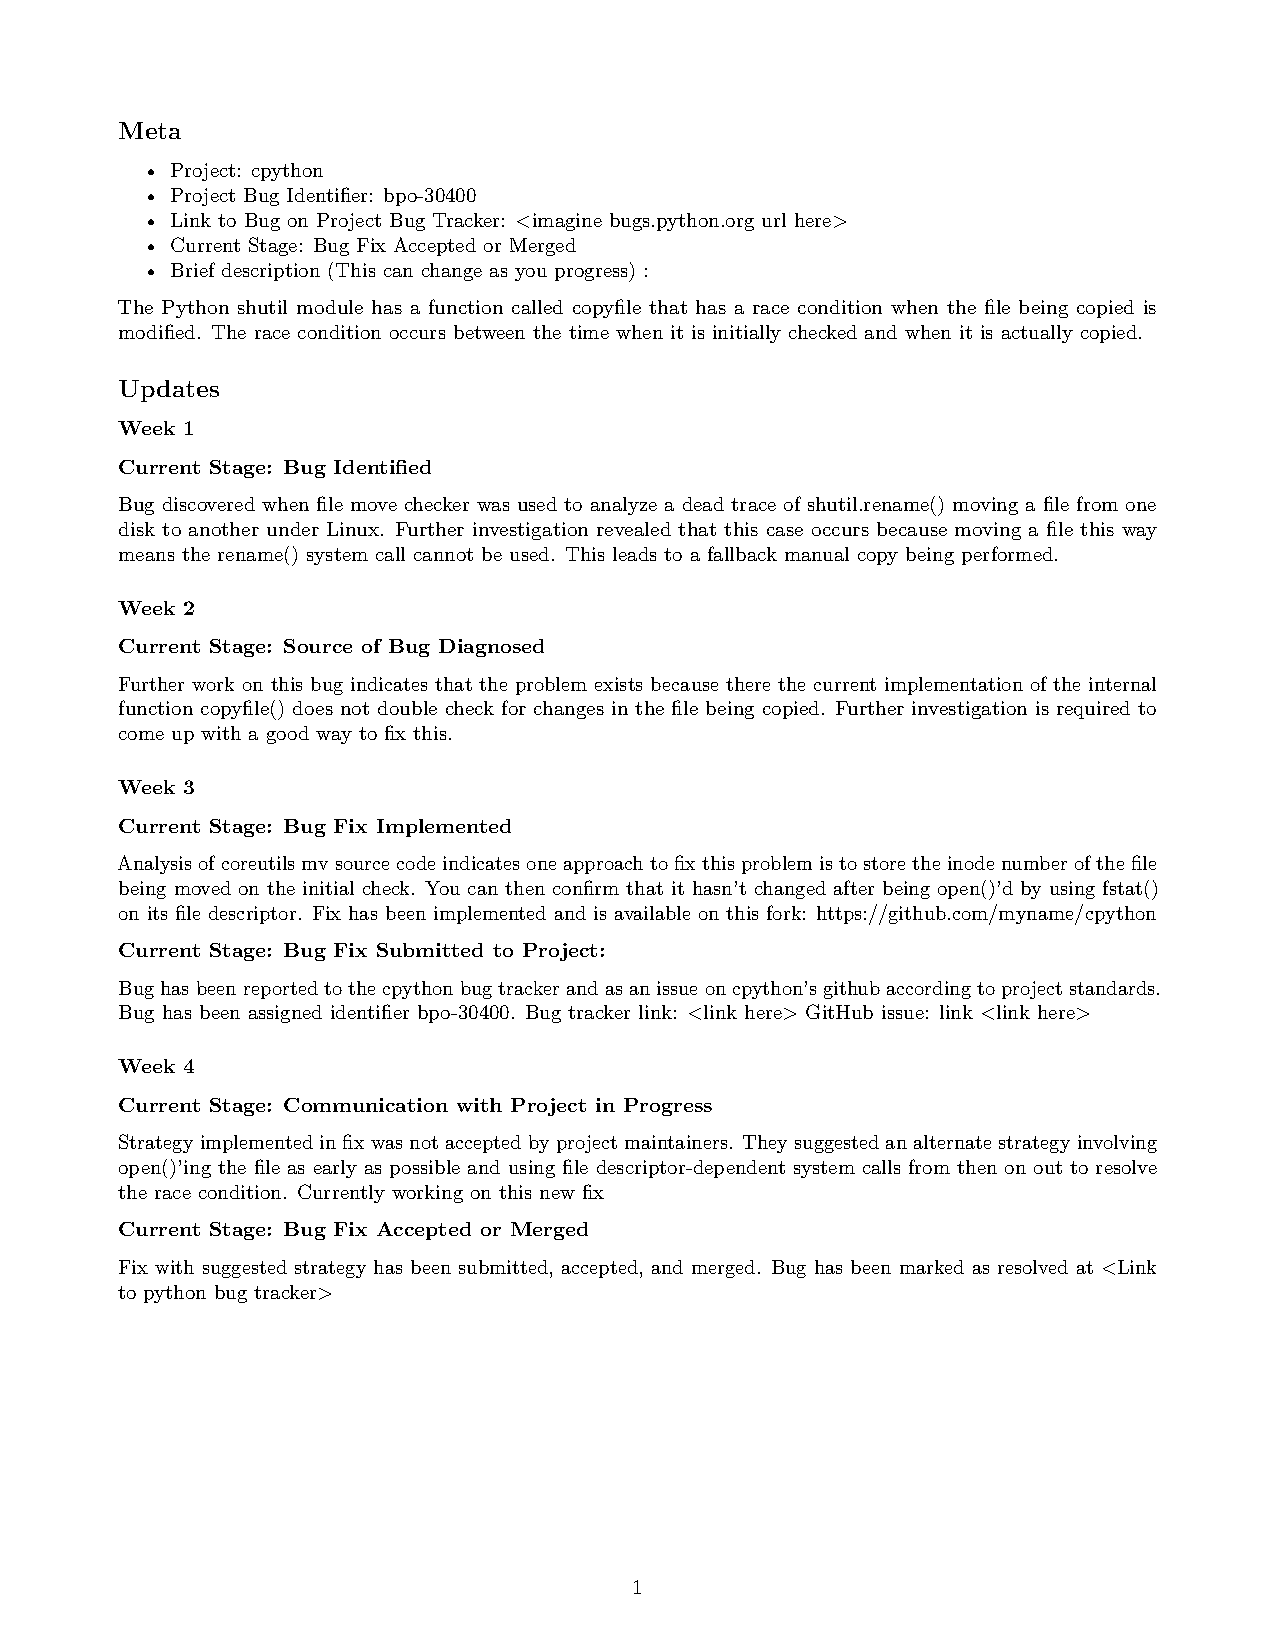
\includegraphics[scale=.8]{chapter5/figures/examplereport}}
\caption[Example Progress Report]{Example Progress Report}
\label{fig:examplereport}
\end{figure}
\restoregeometry

\section{Bugs Found by Participants}
\label{subsec:bugs-by-participants}
Study participants found a total of 18 bugs using CrashSimulator's
``Unusual Filetype Mutator.''
Participants constructed patches to correct six of these bugs and submitted
them to the appropriate maintainers.
An example of one such patch is listed in Figure~\ref{fig:participantpatch}.

Although some of our participants were able to diagnose and fix the bugs they found,
none of their submitted patches were accepted.
There are several specific reasons why this happened:

\paragraph{Patches Submitted to the Wrong Maintainer}
The most common reason for rejection was some participants submitted their patch to the wrong maintainer.
Most were submitted to Ubuntu Linux's main bug tracker, which is intended to manage distribution-specific bugs.
In these cases,
maintainers classified the bugs as ``WONTFIX'' and referred the submitter to the correct upstream project.
This response indicates that our participants were unaware of the relationship between distribution maintainers and application maintainers.
This deficiency makes it clear that  further instruction is needed about the importance of sending patches to the correct place.

\paragraph{Overly Broad Patches}
A second reason that patches were rejected is because they were considered ``overly broad'' by the maintainers that reviewed them.
An example of this case is a patch for ``sort,'' which would disallow it's processing of anything but regular files.
This would break a very common usage of the tool in which a user ``pipes'' in the output of another utility.
Situations like this suggest that the writer did not fully grasp the implications of the patch they constructed.
Typically this is resolved through dialog between the submitter and maintainer with the goal of producing a mutually acceptable patch.
In this specific case, the participant did not follow up further with the maintainer.

\paragraph{``Not A Bug''}
A final common outcome was that patches were rejected because the behavior they intended to fix was determined to be ``not a bug'' by the receiving maintainer.
This opinion stems from varying definitions of ''application misbehavior.''
In our work on the SEA technique and CrashSimulator, we argued that  consuming large amounts of resources or running forever constituted undesireable behavior in an application.
The maintainer in this case argued that such outcomes may be the correct
for some usages.
This is another situation where discussions between the submitter and maintainer would be needed to derive an acceptable fix.

Even though the generated patches were not accepted,
the results remain
important as a confirmation that 
users other than the original development team
can find bugs in real world applications with our tool.
Participants commented that narrowing the source of a bug
down to a particular sequence of system calls
was helpful in itself. Identifying the area of
code responsible for the bug decreased the time required to produce a fix.
Though observations of study participants
confirmed that familiarity with operating systems concepts
made it easier to work with CrashSimulator, even
those without this background were able to identify bugs using the
built-in anomalies.


 \begin{figure}
 \begin{lstlisting}[basicstyle=\ttfamily,gobble=4]
     --- ./coreutils_original/coreutils-8.28/src/uniq.c
     +++ ./src/uniq.c
     @@ -333,6 +333,11 @@
      {
        struct linebuffer lb1, lb2;
        struct linebuffer *thisline, *prevline;
     +  struct stat sb;
     +
     +  stat(infile, &sb);
     +  if (S_ISBLK (sb.st_mode) || S_ISCHR (sb.st_mode))
     +    die (EXIT_FAILURE, errno, "error opening device file %s",
              quotef (infile));

        if (! (STREQ (infile, "-") || freopen (infile, "r", stdin)))
          die (EXIT_FAILURE, errno, "%s", quotef (infile));
\end{lstlisting}
\caption[Participant Submitted Patch]{Example of a patch submitted by a CrashSimulator user study participant.
This patch prevents the coreutils `uniq` utility from processing block devices. }
\label{fig:participantpatch}
\end{figure}

\section{Tool Limitations Identified by Participants}
\label{subsec:crashsim-patches}

One of the benefits of open source software is that it can be maintained and improved by the community of its users.
This user study indicates that CrashSimulator is able to garner this sort of interaction from its users.
Students submitted five patches
to the tool's code over the
course of the study period.
Three of these reports included patches built by the reporting students that directly
corrected a bug.
The remaining two patches fixed issues with the scripts responsible for installing CrashSimulator.

The students also submitted 16 reports identifying unsupported system calls. There were also 17 reported bugs in
existing system call handlers or test orchestration code.
On the one hand, this is encouraging.  The necessity of adding
support for new system calls
indicates that the students were
using CrashSimulator to test a wide variety of new applications.
On the other hand, the number of bug reports not related to system call support
indicates there is still work to be done on the tool.


\section{Instructor Observations}
\label{subsec:tool-shortcomings}
Observations of how students worked  with the tool during the study were also revealing.
First,
it became clear that the tool
lacks a dedicated mechanism
for determining
which application behaviors constitute a ``bug.''
For example, an application's developer
may have intended that an application processing an ``infinitely long'' file should run continuously
until killed by an outside command.
Therefore, that behavior should not be classified as a bug.
Second,
it demonstrated that
simply reporting if an application did or did not change its behavior
in the presence of an anomaly may not provide sufficient data to identify a bug. The specific results that indicate the presence of a bug must be made clearer to the user.
Both of these issues could be corrected 
by improving the tool's output.
Clearer descriptions of a given result
can give a better idea of
if,
and why,
users should be concerned.

To conclude, our user study has revealed both strengths and weakness
of the CrashSimulator tool.
We were encouraged by the fact that students were able to find bugs in and build patches for real world applications.
Thus, we feel our results show CrashSimulator is usable by outside developers even if there is still work to be done in getting these patches accepted. 
We are also pleased with the improvements that came to the tool as a result of the collaboration between study participants and CrashSimulator's developers.
The tool has had numerous bug fixes and usability enhancements as a result of this effort.
We hope that such collaboration will be a cornerstone of the CrashSimulator project as we push for its wider adoption.

